\begin{abstract}
We present a soft gelatin-based hydrogel e-skin capable of detecting up to six simultaneous tactile stimuli, using electrical impedance tomography (EIT) measurements and convolutional neural networks. Our networks are trained on \textit{only} real-world data, for which we present two custom data-collecting end-effectors. These allow multi-touch responses to be measured quickly and autonomously (up to 8 s/datapoint), giving datasets more than 10$\times$ larger than those existing in the literature. To demonstrate the benefits of this approach, we train a non-homogeneous skin to predict `macro-braille' patterns in a 3$\times$2 grid, achieving a 89\% classification accuracy.
\end{abstract}


\section{INTRODUCTION}

A significant challenge in the development of biomimetic robots is the achievement of continuous high resolution sensing over large areas \cite{Shih2020, Liu2022}. Human skins are continuous and flexible, allowing them to conform to any objects being handled, and are capable of discriminating between multiple touch locations on their surface \cite{gellis1977two}. One promising method for replicating this functionality in soft robotic implementations is electrical impedance tomography (EIT) \cite{Barber1984, Cheney1999, Russo2017, xin2023electrical, Alian2023Soft}. When coupled with piezoresistive materials, EIT's ability to reconstruct the conductivity changes of a continuous surface can be used to fabricate sensorized e-skins \cite{Liu2020, Silvera2015Artificial}. However, as additional functionalities - such as healability and temperature sensitivity - are added to the skins, many of the assumptions which underlie traditional EIT reconstruction techniques are lost \cite{TerrynLearning, Georgopoulou2023sensorized, Abdelwahed2022Using}, and data-driven approaches must instead be employed \cite{Wang2015Optimized, wang2020deep}.

Whilst many implementations can be trained to predict tactile stimuli in simulation \cite{Park2022, Park2020ERT}, the Sim2Real gap in the simulation of functional materials can be altogether avoided by training on only real-world data \cite{Howison2021, hardman2023tactile}. Though it is straightforward to automate a pressing mechanism which collects and validates single-point presses for training \cite{TerrynLearning, Hardman20223D}, there are few examples of multi-touch skins being trained in this way. Many works validate analytic or pre-trained EIT models by manually placing multiple objects on the skins' surfaces, though this approach cannot be used for large-scale data collection \cite{Zhang2023, Soleimani2022Ionic, Zheng2018}. Others - including the authors' previous work - employ multiple probes with a fixed separation, limiting the variability of data which can be collected \cite{hardman2023tactile, Chen2023Novel, Jamshidi2023EIT}. Park et al. present an EIT \& CNN-based skin trained in silico which is capable of multi-touch responsivity \cite{Park2022}, though only demonstrate this responsivity qualitatively, due to a lack of a physical multi-touch dataset. The authors are aware of only one such dataset in the EIT skin literature: Duan et al. manually position 252-point two-object measurements for their conductive fabric EIT sensor \cite{Duan2019}.

\begin{figure}[htbp]
  \centering
  \includegraphics[width=\linewidth]{Images/MultiTouchIntro.pdf}
  \caption{Automated collection of physical multi-touch datasets for EIT-based e-skins. (a) Measurements are taken from 32 electrodes surrounding a rectangular hydrogel e-skin. (b) Our two-point prober, with controllable probe separation, angle, and activation. (c) Our six-point prober, used to apply customizable macro-braille patterns to the e-skin.}
  \label{fig:intro}
\end{figure}

% Gelatin-based hydrogels are being increasingly used in soft robotic applications, demonstrating highly desirable flexibility, stretchability, environmental sensitivity, healability, tunability, and printability \cite{Heiden2022, Hardman2022, baumgartner2020resilient}. However, these additional functionalities, coupled with the nonlinearities of EIT's inverse problem \cite{Khan2019, Santosa1990}, causes difficulties in their analytic reconstructions from EIT hardware \cite{hardman2023tactile}.

In this work we explore the data-driven multi-touch responsivity of a functional gelatin-glycerol hydrogel e-skin, presenting two automated probing end effectors which can straightforwardly collect data from multiple points. Using these large datasets of up to 3200 points, we compare different methods of localization and investigate the nonlinear superpositions of two-point probing, using machine learning approaches to overcome the material's difficulties in analytic reconstructions \cite{hardman2023tactile}. We end by using a non-homogeneous skin to classify large-scale braille letters pressed into its surface, achieving a 89\% success rate.

Since this real-world data collection method allows us to collect a much larger physical multi-point dataset than anything existing in the EIT-based e-skin literature, we end by discussing its implications for the validation and benchmarking of future developments.

\section{MATERIALS \& METHODS} \label{sec:methods}

Two multi-touch end effectors are validated on a rectangular hydrogel e-skin, shown in Figure \ref{fig:intro}a. This is secured within a two-part laser cut acrylic frame, which presses 32 equally spaced stainless steel M4 bolts into its perimeter, which function as electrodes during tomography measurements. These measurements and the skin's fabrication process are described in detail at the end of this section.

To gather multi-touch datasets, a \textit{Universal Robots} UR5 robot arm is fitted with two custom end effectors. Both can push a specified combination of 3D printed polylactic acid (PLA) probes with 5 mm diameter into the skin's surface. We measure the changes in conductivity arising from material strains, and therefore use insulating probes to minimize the effects of exogeneous substances.

The first prober (Figure \ref{fig:intro}b) can be used for both one and two point data collection, since one probe can be withdrawn using a servo motor-driven rack and pinion. A second pinion gear controls the separation distance of the two probes. If both probes are fully extended, the system therefore has 5 degrees of freedom: the $x$ \& $y$ coordinates of both, and the depth to which they are pressed. The UR5 controls translational and rotational motion, with our additional mechanical system enabling all five degrees to be realized. Conversely, if the adjustable probe is withdrawn, only 3 coordinates ($x$, $y$, \& depth) of the fixed probe are necessary. 

During data collection, the in-plane degrees of freedom ($x$ \& $y$) are randomised within the skin, enforcing a 'deadzone' of 10 mm around the internal perimeter of the frame to avoid collisions. Depths are set to fixed values, as described in Section \ref{sec:results}, and all probes are kept perpendicular to the plane of the skin.

The second multi-touch end effector facilitates up to six simultaneous presses, and is shown in Figure \ref{fig:intro}c. Each of the probes can be extended via a servo-driven rack \& pinion mechanism, determined via a binary string sent serially to the Arduino Mega 2560 which acts as the controller. The setup is designed to be modular: each probe can be bolted to any location on a laser cut acrylic pegboard, with holes at 15 mm increments. Throughout the experiments in Section \ref{sec:results}, the probes are arranged in a `macro-braille' configuration: a 3$\times$2 grid with 45 mm probe separation. 

The skin's response to probing is recorded using a 32-input \textit{EIT-kit}, as described by Zhu et al. \cite{Zhu2021EIT}. Adjacent excitation and measurement pairs are selected, giving a total of 928 non-overlapping tetrapolar electrode configurations. An update of every channel occurs every 100 ms: by averaging 5 frames at a time, the hardware returns data at a rate of 2 Hz. The acrylic frame's stainless steel electrodes are attached to the board's multiplexer via alligator leads and a 34-channel breakout, as shown in Figure \ref{fig:intro}.

% processing/ML/CNN architectures

The datasets are split into 80:10:10 train-validation-test sets, and standardised in all models.

Three machine learning model architectures are trained on single point data: a ridge regression model, a fully-connected (FC) feedforward neural network, and a convolutional neural network (CNN) whose output is a $ 6\times8 $ discretised grid of possible touch positions. 

The ridge regression model pipeline used standard scaled data, applied principal component analysis with 100 principal components to retain 93\% of the variance, and performed least-squares polynomial (order 2) regression with $ L^2 $ regularisation. Cross-validation with 5 folds and a grid search over a range of regularisation trade-off coefficients ($\alpha$) were applied. 

The fully-connected neural network (FCNN) used two hidden layers with 256 and 32 neurons, each with a ReLU activation function, and an output layer of 2 neurons for an $(x, y)$ predicted touch coordinate with no activation. The model was compiled with an Adam optimiser and a mean-squared error loss function.

The convolutional neural network (CNN) took in the data as a $ 32 \times 32 $ array. It used two hidden layers with 256 and 64 neurons with square kernels of size $ 3 \times 3 $ and $ 7 \times 7 $ respectively, each with ReLU activations. Downsampling via max pooling with a $ 2 \times 2 $ pool size was applied to the output of this layer, followed by regularisation by a dropout layer at a rate of 0.25. Two fully-connected hidden layers with 128 and 48 neurons were added, with ReLU and sigmoid activations respectively, such that the output could be represented as a $ 6 \times 8 $ array of binary classification confidences. The model was compiled with an Adam optimiser and a binary cross-entropy loss function. This network was used to predict multi-touch locations. In both the FCNN and the CNN, hyperparameter optimisation via a Bayesian algorithm was used to determine these parameters after 10 trials by selecting models with the best validation loss.

A copy of the Jupyter Notebook used to carry out the analysis is provided at the end of this manuscript.

Figure \ref{fig:2point}'s analytic reconstructions are performed using EIDORS' one-step Gauss-Newton implementation with a Laplace prior \cite{Adler_2006}.

% e-skin details

The conductive hydrogel skin is formed by mixing 240 bloom pork gelatin powder \textit{(MM Ingredients)}, glycerol \textit{(Fisher Scientific)}, water, citric acid monohydrate \textit{(Fisher Scientific)}, and sodium chloride \textit{(Fisher Scientific)} by weight ratio 1 : 1.5 : 2.5 : 0.2 : 0.1, as described by Hardman et al. \cite{Hardman2022}. The mixture is stirred and incubated in a water bath at 50 $^{\circ}$C for two hours before pouring into a rectangular acrylic mould with internal dimensions 180 $\times$ 120 $\times$ 3 mm. Upon solidifying, the skin is clamped loosely into the 120 $ \times $ 80 mm acrylic frame; as its water content comes to equilibrium with the environment, it is then held in tension. The frame is fixed to a PLA base using 4 M6 bolts. Beneath the skin, a 30 mm deep silicone \textit{(EcoFlex 00-10)} substrate is cast, into which the skin can be pressed by the probes. Figure \ref{fig:forces}'s force measurements are recorded using a \textit{Kern EMS} balance positioned underneath the frame during probing.

To highlight the ability of our approach to collect data for non-homogeneous skins, the experiments in Figures \ref{fig:singledata} \& \ref{fig:6point} use variable conductivity patterns printed onto the skin. These are composed of the same hydrogel as the base layer, with additional carbon black \textit{(Fisher Scientific)} added by 0.25:1 weight ratio to the gelatin powder. Two grid patterns are used: 2$\times$1 \& 3$\times$2, both of which can be seen on the skin in Figure \ref{fig:intro}. These are fabricated using a \textit{Wiiboox LuckyBot} extruder heated to 45$^\circ$C on a \textit{Creality CR20} frame.

All microcontroller programming is done in C++, using the PlatformIO environment in Visual Studio Code. All other programming uses Python, using TensorFlow/Keras with Jupyter Notebooks for machine learning and serial communications for robot and Arduino interfacing.

% An identical robot and plastic finger setup was used for all trials. Considerable noise from the EIT data was seen in all measurements, making analytic reconstruction challenging. During preliminary testing, it was observed that using one's real finger to press the skin produced far larger signals than those of to the plastic fingers, presumably due to the presence of the natural conductive oils (sebum) on the surface of the fingers.

\section{RESULTS \& DISCUSSION} \label{sec:results}

We first validate the single-point responsiveness of the raw signals returned from the e-skin over different locations, depths, and electrode configurations. The responses for three electrode combinations (\textcircled{\raisebox{-.9pt} {1}}, \textcircled{\raisebox{-.9pt} {2}} \& \textcircled{\raisebox{-.9pt} {3}} from Figure \ref{fig:intro}a) and locations (\textbf{A}, \textbf{B} and \textbf{C} from Figure \ref{fig:intro}a) are shown in Figure \ref{fig:single} for pressing depths of 4, 8 \& 12 mm. Their corresponding forces are plotted in Figure \ref{fig:forces}, where it is clear that the resistance is dominated by the silicone substrate.

\begin{figure}[htbp]
  \centering
  \includegraphics[width=\linewidth]{Images/SingleResponse.pdf}
  \caption{Single-point responsivity, for three probing depths (4, 8 \& 12 mm) at the selected points (A, B \& C) and electrode combinations (\textcircled{\raisebox{-.8pt} {1}}, \textcircled{\raisebox{-.8pt} {2}} \& \textcircled{\raisebox{-.8pt} {3}}).}
  \label{fig:single}
\end{figure}

Figure \ref{fig:single}'s top row shows the maximum deviation in voltage response in the duration of pressing from the time-averaged unpressed baseline, for each press site, electrode combination, and depth. In most cases, the response increases with press depth, supporting the idea that the hydrogel's strain is responsible for its impedance changes. However, these raw magnitudes are highly susceptible to noise, which can be seen in the two selected lower row time-series (\textbf{B}, \raisebox{.5pt}{\textcircled{\raisebox{-.9pt} {3}}}, 12 mm \& \textbf{C}, \raisebox{.5pt}{\textcircled{\raisebox{-.9pt} {2}}}, 8 mm). Despite having similar maximum deviations from the baseline, the latter responds much more strongly within the pressed (green) zones, and it seems that data-smoothing is required to reliably identify these responses. As such, data-smoothing is integrated from Figure \ref{fig:2point} onwards.

\begin{figure}[htbp]
  \centering
  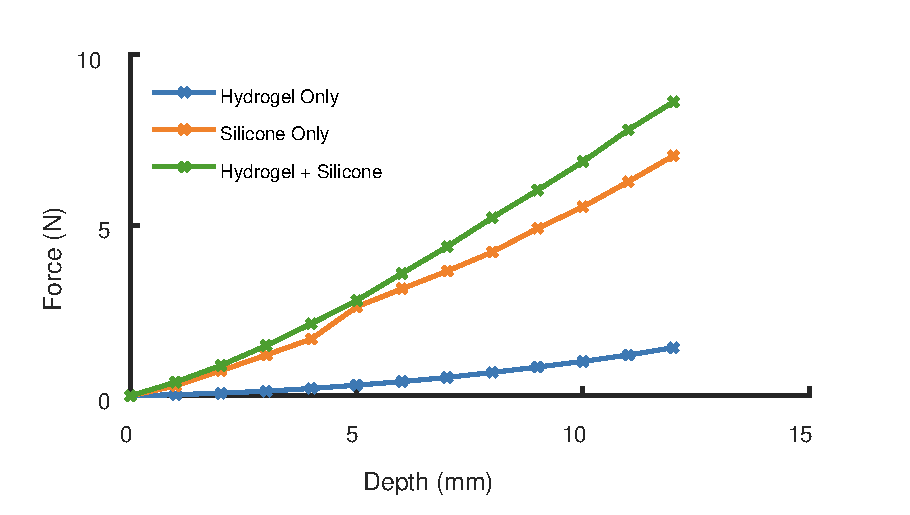
\includegraphics[width=\linewidth]{Images/ForceFig.eps}
  \caption{Force vs pressing depth for the silicone block, hydrogel e-skin, and combined system.}
  \label{fig:forces}
\end{figure}

However, since physically collecting sufficient data for smoothing slows the process, we also show that machine learning approaches can reasonably deal with the signal noises from fast data collection: learning to localize tactile stimuli with just one frame of data before and after each press. To do so, we collect 3 single-point datasets from 3 skins (homogeneous, low conductivity printed grid, high conductivity printed grid) at a fixed depth of 10 mm, with sizes 3200, 550 and 550 respectively. Three architectures (described in Section \ref{sec:methods}: ridge regression, feedforward neural network and convolutional neural network with a discretized output) are trained on their noisy signals. Figure \ref{fig:singledata} plots their predictions for a selected set of points from the training set.

Of the two single-point predicting networks, the fully-connected approach performs best, with the ridge-regression model commonly converging to predict the centermost point. The fully-connected network can give good localization predictions from the noisy single-frame responses for the homogeneous skin. However, this architecture is difficult to extend to multi-touch scenarios, where the total number of predicted points is unknown. To address this, we also test a convolutional neural network (CNN) which returns a confidence value that each `tile' in a grid is being touched. Since this approach can be verified even with Figure \ref{fig:single}'s noisy data, a grid-based CNN prediction is selected for later 6-point experiments.  

\begin{figure}[htbp]
  \centering
  \includegraphics[width=\columnwidth]{Images/SingleData.pdf}
  \caption{Randomly selected single-point predictions, using different skin compositions and training methods.}
  \label{fig:singledata}
\end{figure}

The two neural networks do not perform as well with the non-homogeneous skins, though patterns are still detected in the data which enable non-central points to be predicted. After smoothing the responses, we choose to perform our final tests using a high conductivity grid, to demonstrate the robustness of our multi-point data collection methods.

% This is likely because the press site is much further from the selected electrodes, so the displacement has no effect on the local impedance of the e-skin. The results in the top row for these cases are taken from the last of the five trials.

% To reduce the noise, the microcontroller collecting the EIT data applied an average over five samples at each time step, although considerable noise remained in our data even after this smoothing.

Having validated our single-touch data, we move to the collection of multi-point datasets. Table \ref{tab:speeds} shows the speeds at which these can be physically collected using our custom setup - such datasets enable the multi-touch responses of complex skin shapes and compositions to be automatically mapped, with no Sim2Real gap. As an example, we use the two-point prober to demonstrate the nonlinearity of the hydrogel skin's responses during multi-touch pressing, before using a CNN approach to overcome these difficulties in a final `macro-braille' demonstration. For the former, Figure \ref{fig:2point}'s first column illustrates the output of a one-step analytic reconstruction fed a two-point press at 5 mm depth. Patterns are visible, with the central blue feature being biased towards the probed areas in each case, but it is difficult to extract locations. If an unknown number of probed points were used, predicted press locations become more uncertain, and machine-learning approaches (such as the CNN of Figure \ref{fig:singledata}) are favored.

\begin{table}[htbp]
    \centering
    \caption{Datasets collected by the automated end effectors, and the average time per datapoint.}
        \begin{tabular}{|c|c|c|}
        \hline
        \textbf{Description} & \textbf{Size} & \textbf{T$_{average}$ (s)} \\
        \hline
        1-point, no smoothing & 3200 & 5\\
        2-point, no smoothing & 1600 & 7\\
        2-point, highly smoothed & 50 & 11\\
        6-point, smoothed & 1100 & 8\\
        \hline
        \end{tabular}
    \label{tab:speeds}
\end{table}

\begin{figure}[htbp]
  \centering
  \includegraphics[width=\columnwidth]{Images/bitmap.png}
  \caption{Multi-touch: the 2-point prober is used to probe two individual locations, both separately and together. One-step analytic reconstructions of the combined response are also shown.}
  \label{fig:2point}
\end{figure}

The reason behind these reconstruction difficulties can be seen in Figure \ref{fig:2point}'s bar plots, which plot the smoothed response magnitudes of two representative electrode combinations to the press combinations. Using the custom end effector, three situations are plotted for each: the response of each individual point (blue \& orange), and the two simultaneously (green). Each press type is repeated five times: error bars illustrate the total range of the response, with mean values represented by the bars themselves. Case (a) behaves as might be expected: both electrode combinations respond to both press locations, and the combined response is correspondingly the largest. Still, the values do not follow a linear superposition, suggesting that real-world multi-touch data is required before such press depths can be reliably predicted for previously unseen cases. 

Conversely, case (b) does not behave in this way. Both electrode combinations respond well to the press at location 1 and give only a small response at location 2, as could be qualitatively predicted by plotting lines-of-least-resistance between the injection and measurement electrodes. However, the combined response is slightly \textit{lower} for both electrode combinations; such effects cannot be predicted without an accurate model of the hydrogel's conductivity mechanisms, or a learnt model from prior experiences.

Finally, case (c) behaves differently for the two electrode combinations: on the left hand side, the combined response is between the two individual response magnitudes, whilst on the right hand side the combined response has the greatest magnitude. Using the custom two-point prober, these patterns can be identified and accounted for during predictions.

To validate this, we demonstrate how the complete system can identify large-scale braille patterns from Figure \ref{fig:intro}c's 6-point prober, trained using only experimentally-collected real-world data; the speed of collection is quantified in Table \ref{tab:speeds}. We use Figure \ref{fig:singledata}'s high conductivity grid, showing that our approach is possible beyond the scope of homogeneous skins.

\begin{figure*}[htbp]
  \centering
  \includegraphics[width=0.85\linewidth]{Images/Architecture.pdf}
  \caption{6-point (`macro-braille') data collection and prediction. \textcolor{red}{Not sure this is the architecture behind final figs.}}
  \label{fig:architecture}
\end{figure*}

Figure \ref{fig:architecture} maps the data collection and training process: a UR5 robotic arm supports the prober above the skin. Random noise in the range $\pm$8 mm is added to the translational position before each press, avoiding convergence of the solution to specific locations of the probes. 1100 random combinations of probe positions are collected, each encoded as a 6-bit binary string. For each, the skin's 928-channel response is measured and smoothed, used as the input to a convolutional neural network, which is trained to map the standard-scaled, time-averaged EIT measurements $ \mathbf{x} \in \mathbb{R}^{1024} $ into the tile touch predictions $ \mathbf{y} \in \mathbb{R}^{6} $, where $ 0 \leq y_i \leq 1, \ \forall i \in \left \{  0 ... 5\right \} $. These 6 predictions can be displayed as a `braille output' grid to visualize the certainty levels, or can further undergo binary thresholding (rounding to the nearest integer), to predict whether each of the 6 probes is extended or retracted.

\begin{figure}[htbp]
  \centering
  \includegraphics[width=\columnwidth]{Images/6pointdata.pdf}
  \caption{a) Visualisations of the CNN predictions and ground truth braille patterns randomly selected from the training and test sets. b) Identification rates of the binary outputs for individual tiles and full patterns.}
  \label{fig:6point}
\end{figure}

Figure \ref{fig:6point}a plots 4 random selections from the training and test sets data of the CNN. Red crosses (${\textcolor{red}{\times}}$) mark the ground truth for each test i.e. which of the tiles were pressed. Though the `braille output' (see Figure \ref{fig:architecture}) is plotted, the network tends towards near-binary outputs, with only one of the test set squares noticably falling in the uncertainc central region. Here, this near-white tile (test sample 4) is correctly classified as unpressed despite its higher uncertainty. The performances of the network throughout the entire training and test sets are given in Figure \ref{fig:6point}b, split into `individual tile' and `six-tile pattern' cases. Both rely on Figure \ref{fig:architecture}'s binary output: in the former, the successful classification rate for any tile (97.6\% in the test set) is considered, whilst the latter quantifies the proportion of 6-tile grids which are classified entirely correctly - in the test set, this occurs 89\% of the time. Scaling the membrane to fingertip size could therefore provide a high classification rate for braille reading trained only on real-world data, with the potential for improvement using contextful information from words and letters. In addition, since the skin is entirely sensorized, such a system would not be limited to only predict 6 stimuli: any conductivity-changing effect could also be measured.

\section{CONCLUSIONS}
In this work we have demonstrated \& validated the use of automated multi-point data collection for EIT-based e-skins, using two novel end-effectors. With no Sim2Real gap, we physically collect multiple EIT datasets of sizes up to 3200, more than 10$\times$ larger than existing manually-collected datasets (252). Multi-touch data points can be collected as quickly as 8 s per frame, facilitating the generation of large numbers of known responses for complex shapes and enabling data-driven responses. We demonstrate tactile localization at the highest speeds of data collection, and use an automated prober to explore the nonlinear superposition behaviours of a functional hydrogel e-skin to multiple presses. Finally, we train the e-skin's CNN to recognize macro-braille patterns with an 89\% success rate, using only real-world data with added noise.

These results act as a preliminary demonstration of the merits of physical multi-touch data for EIT e-skins using automatically collected data. The repeatability of these custom probers can be used to develop multi-touch benchmarks which enable better characterization between skins, and can be run for prolonged periods of time without manual intervention. Furthermore, patterns in the response behaviors of functional materials can be autonomously identified and characterized, accelerating their integration into soft robotic applications.
